\section{Policy Learning Details}
\label{sec:supp-lqr}

Given a TVLG dynamics model and quadratic cost approximation, we can approximate our Q and value functions to second order with the following dynamic programming updates, which proceed from the last time step $t = T$ to the first step $t = 1$:
\begin{align*}
    Q_{\mathbf{s},t}=c_{\mathbf{s},t}&+\dynmat_{\mathbf{s},t}^\top{V}_{\mathbf{s},t+1}\,,~~Q_{\mathbf{ss},t}=c_{\mathbf{ss},t}+\dynmat_{\mathbf{s},t}^\top{V}_{\mathbf{ss},t+1}\dynmat_{\mathbf{s},t}\,,\\
    Q_{\mathbf{a},t}=c_{\mathbf{a},t}&+\dynmat_{\mathbf{a},t}^\top{V}_{\mathbf{s},t+1}\,,~~Q_{\mathbf{aa},t}=c_{\mathbf{aa},t}+\dynmat_{\mathbf{a},t}^\top{V}_{\mathbf{ss},t+1}\dynmat_{\mathbf{a},t}\,,\\
    &Q_{\mathbf{sa},t}=c_{\mathbf{sa},t}+\dynmat_{\mathbf{s},t}^\top{V}_{\mathbf{ss},t+1}\dynmat_{\mathbf{a},t}\,,\\
    &V_{\mathbf{s},t}=Q_{\mathbf{s},t}-Q_{\mathbf{sa},t}Q_{\mathbf{aa},t}^{-1}Q_{\mathbf{a},t}\,,\\
    &V_{\mathbf{ss},t}=Q_{\mathbf{ss},t}-Q_{\mathbf{sa},t}Q_{\mathbf{aa},t}^{-1}Q_{\mathbf{as},t}\,.
\end{align*}
It can be shown (e.g., by \citet{synthesis}) that the action $\mathbf{a}_t$ that minimizes the second-order approximation of the Q-function at every time step $t$ is given by
\[
\mathbf{a}_t=-Q_{\mathbf{aa},t}^{-1}Q_{\mathbf{as},t}\mathbf{s}_t-Q_{\mathbf{aa},t}^{-1}Q_{\mathbf{a},t}\,.
\]
This action is a linear function of the state $\mathbf{s}_t$, thus we can construct an optimal linear policy by setting $\mathbf{K}_t=-Q_{\mathbf{aa},t}^{-1}Q_{\mathbf{as},t}$ and $\mathbf{k}_t=-Q_{\mathbf{aa},t}^{-1}Q_{\mathbf{a},t}$. We can also show that the maximum-entropy policy that minimizes the approximate Q-function is given by
\[
\pi^\star(\mathbf{a}_t|\mathbf{s}_t)=\mathcal{N}(\mathbf{K}_t\mathbf{s}_t+\mathbf{k}_t,Q_{\mathbf{aa},t}).
\]
Furthermore, as in \citet{mfcgps}, we can impose a constraint on the total KL-divergence between the old and new trajectory distributions induced by the policies through an augmented cost function $\tilde{\cost}(\state_t,\action_t)=\frac{1}{\lambda}\costmodel(\state_t,\action_t)-\log\bar{\policy}(\action_t|\state_t)$, where solving for $\lambda$ via dual gradient descent can yield an exact solution to a KL-constrained LQR problem.


\section{Parameterizing the Cost Model}
\label{sec:supp-cost}

The simplest choice that we consider for parameterizing the cost model is as a full quadratic function of the state and action, i.e.,     $\costmodel(\state_t,\action_t)=\frac{1}{2}\state_t^\top\costmat\state_t+\costvec^\top\state_t+\alpha\|\action_t\|_2^2+b$ where we assume that the action-dependent part of the cost -- i.e., $\alpha$ -- is known, and we impose no restrictions on the learned parameters $\costmat$ and $\costvec$. This is our default option due to its simplicity and the added benefit that fitting this model locally can be done in closed form through least-squares quadratic regression on the observed states. However, another option we consider is to choose $\costmodel(\state_t,\action_t)=\frac{1}{2}\state_t^\top\mathbf{L}\mathbf{L}^\top\state_t+\costvec^\top\state_t+\alpha\|\action_t\|_2^2+b$. $\mathbf{L}$ is a lower-triangular matrix with non-negative diagonal entries, and thus by constructing our cost matrix as $\costmat=\mathbf{L}\mathbf{L}^\top$ we guarantee that the learned cost matrix is positive semidefinite, which can improve the behavior of the policy update.

In general, in this work, we consider quadratic parameterizations of the cost model since we wish to build a LQS model. However, in general it may be possible to use non-quadratic but twice-differentiable cost models, such as a neural network model, and compute local quadratic cost models using a second-order Taylor approximation as in \citet{mfcgps}. We also do not assume access to a goal observation, though if provided with such information we can use construct a quadratic cost function that penalizes distance to this goal in the learned latent space, as in \citet{spatial-ae} and \citet{e2c}.


\section{The SVAE Algorithm}
\label{sec:supp-svae}

\citet{Johnson2016} builds off of \citet{Hoffman2013} and \citet{Winn2005}, who show that, for conjugate exponential models, the variational model parameters can be updated using natural gradients of the form
\begin{equation}
    \tilde{\nabla}_{\omega}\mathcal{L}=\omega^0+B\mathbb{E}_q\left[t_{\dynmat,\dyncovar}(\dynmat,\dyncovar)\right]-\omega\,,
\end{equation}
Where $\omega$ denotes the MNIW parameters of the variational factors on $\dynmat,\dyncovar$, $B$ is the number of minibatches in the dataset, $\omega^0$ is the parameter for the prior distribution $p(\dynmat,\dyncovar)$, and $t_{\dynmat,\dyncovar}(\dynmat,\dyncovar)$ is the sufficient statistic function for $p(\dynmat,\dyncovar)$. Thus, we can use this equation to compute the natural gradient update for $\omega$, whereas for $\gamma$, $\phi$, and the parameters of the cost model, we use stochastic gradient updates on Monte Carlo estimates of the ELBO, specifically using the Adam optimizer \citep{Kingma2013}. This leads to two simultaneous optimizations, and their learning rates are treated as separate hyperparameters. We have found $10^{-4}$ and $10^{-3}$ to be good default settings for the natural gradient step size and stochastic gradient step size, respectively.


\section{Fitting the Local Dynamics Model}
\label{sec:supp-fit}

In the pretraining phase described in \autoref{sec:solar-modeling}, we are learning the following sets of parameters from observed trajectories:
\vspace{-.5em}
\begin{enumerate}
    \itemsep0em
    \item The parameters of the variational posterior over global dynamics $q_\textrm{global}(\dynmat, \dyncovar)$;
    \item The weights of the encoder and decoder networks $\decoder_\gamma(\state)$ and $\encoder_\phi(\observation)$;
    \item The parameters of the cost function $\costmodel(\state, \action)$.
\end{enumerate}
\vspace{-.5em}
In the RL phase described in \autoref{sec:inference}, after learning the representation and global models, we fit local, linear-Gaussian dynamics models to additional trajectories. The conjugacy of the Bayesian LQS model enables a computationally efficient expectation-maximization procedure to learn the local dynamics. We assume the same graphical model as in \autoref{eq:gm-start} to \autoref{eq:gm-end} except we modify \autoref{eq:dyn} and \autoref{eq:dyn2} to be
\begin{align*}
    \dynmat_t, \dyncovar_t &\sim p(\dynmat_t, \dyncovar_t) \triangleq q_{\textrm{global}}(\dynmat, \dyncovar)\,,\\
    \state_{t + 1} | \state_t, \action_t, \dynmat_t, \dyncovar_t &\sim \N(\dynmat_t\colvec{\state_t\\\action_t}, \dyncovar_t)\,.
\end{align*}
The model assumes that the TVLG dynamics are independent samples from our global dynamics, followed by a deep Bayesian LDS to generate trajectories. This is similar to the globally trained model, with the exception that we explicitly assume time-varying dynamics.

Now suppose we have collected a set of trajectories of the form $\trajectory$ and aim to fit a local dynamics model. We use variational inference to approximate the posterior distributions by setting up the variational factors
\vspace{-.5em}
\begin{enumerate}
    \itemsep0em
    \item $q(\state_{1:\horizon} | \dynmat_{1:\horizon}, \dyncovar_{1:\horizon}; \observation_{1:\horizon}, \action_{1:\horizon})$, which approximates the posterior distribution $p(\state_{1:\horizon} | \observation_{1:\horizon}, \action_{1:\horizon}, \dynmat_{1:\horizon}, \dyncovar_{1:\horizon})$;
    \item $q(\dynmat_t, \dyncovar_t)$, which approximates the posterior distribution $p(\dynmat_t, \dyncovar_t | \state_{1:\horizon}, \action_{1:\horizon})$
\end{enumerate}
\vspace{-.5em}
The ELBO under these variational factors is:
\begin{align*}
    \mathcal{L} &= \mathbb{E}_q \big[\sum_t^\horizon \log p(\observation_t | \state_t)\\ &- \mathrm{KL}\left(q(\state_{1:\horizon})\|p(\state_{1:\horizon} | \action_{1:\horizon}, \dynmat_{1:\horizon}, \dyncovar_{1:\horizon})\right)\\
    &- \sum_t^{\horizon - 1} \mathrm{KL}\left(q(\dynmat_t, \dyncovar_t)\|p(\dynmat_t, \dyncovar_t)\right)
    \big]
\end{align*}

We use variational EM to alternatively optimize $q(\state_{1:\horizon} | \dynmat_{1:\horizon}, \dyncovar_{1:\horizon}; \observation_{1:\horizon}, \action_{1:\horizon})$ and $q(\dynmat_t, \dyncovar_t)$. Using evidence potentials $\psi(\state_t;\observation_t,\phi)$ output by the recognition network $\encoder_\phi(\observation_t)$, both of these optimizations can be done in closed form. Specifically, the optimal $q(\state_{1:\horizon} | \dynmat_{1:\horizon}, \dyncovar_{1:\horizon}; \observation_{1:\horizon}, \action_{1:\horizon})$ is computed via Kalman smoothing using evidence potentials from the recognition network, and the optimal $q(\dynmat_t, \dyncovar_t)$ can be computed via Bayesian linear regression using expected sufficient statistics from $q(\state_{1:\horizon} | \dynmat_{1:\horizon}, \dyncovar_{1:\horizon}; \observation_{1:\horizon}, \action_{1:\horizon})$.


\section{Experiment Setup}
\label{sec:supp-set}

{\bf 2D navigation.} Our recognition model architecture for the 2D navigation domain consists of two convolution layers with \mbox{2-by-2} filters and 32 channels each, with no pooling layers and ReLU non-linearities, followed by another convolution with \mbox{2-by-2} filters and 2 channels. The output of the last convolution layer is fed into a fully-connected layer which then outputs a Gaussian distribution with diagonal covariance. Our observation model consists of FC hidden layers with 256 ReLU activations, and the last layer outputs a categorical distribution over pixels. We initially collect 100 episodes which we use to train our model, and for every subsequent RL iteration we collect 10 episodes. The cost function we use is the sum of the $L^2$-norm squared of the distance to the target and the commanded action, with weights of 1 and 0.001, respectively.

As discussed in \autoref{sec:solar-experiments}, we modify the 2D navigation task from \citet{e2c} and \citet{rce} to randomize the location of the target every episode, and we set this location uniformly at random between $-2.8$ and $2.8$ for both the x and y coordinates, as coordinates outside of $[-3,3]$ are not visible in the image. We similarly randomize the initial position of the agent. In this setup, we use two \mbox{32-by-32} images as the observation, one with the location of the agent and the other with the location of the target, and in the fixed-target version of the task we only use one \mbox{32-by-32} image.

{\bf Nonholonomic car.} The nonholonomic car domain consists of \mbox{64-by-64} image observations. Our recognition model is a convolutional neural network with four convolutional layers with \mbox{4-by-4} filters with 4 channels each, and the first two convolution layers are followed by a ReLU non-linearity. The output of the last convolutional layer is fed into three FC ReLU layers of width 2048, 512, and 128, respectively. Our final layer outputs a Gaussian distribution with dimension 8. Our observation model consists of four FC ReLU layers of width 256, 512, 1024, and 2048, respectively, followed by a Bernoulli distribution layer that models the image. For this domain, we collect 100 episodes initially to train our model, and then for RL we collect 100 episodes per iteration. The cost function we use is the sum of the $L^2$-norm squared of the distance from the center of the car to the target and the commanded action, with weights of 1 and 0.001, respectively.

{\bf Reacher.} The reacher domain consists of \mbox{64-by-64-by-3} image observations. Our recognition model consists of three convolutional layers with \mbox{7-by-7}, \mbox{5-by-5}, and \mbox{3-by-3} filters with 64, 32 and 8 channels respectively. The first convolutional layer is followed by a ReLU non-linearity. The output of the last convolutional layer is fed into an FC ReLU layer of width 256, which outputs a Gaussian distribution with dimension 10. Our observation model consists of one FC ReLU layers of width 512, followed by three deconvolutional layers with the reverse order of filters and channels as the recognition model. This is followed by a Bernoulli distribution layer that models each image. We collect 200 episodes initially to train our model, and then for RL we collect 100 episodes per iteration. The cost function we use is the sum of the $L^2$-norm of the distance from the fingertip to the target and the $L^2$-norm squared of the commanded action, which is the negative of the reward function as defined in Gym.

{\bf Sawyer Lego block stacking.} The image-based Sawyer block-stacking domain consists of \mbox{64-by-64-by-3} image observations. The policy outputs velocities on the end effector in order to control the robot. Our recognition model is a convolutional neural network with the following architecture: a \mbox{5-by-5} filter convolutional layer with 16 channels followed by two convolutional layers using \mbox{5-by-5} filters with 32 channels each. The convolutional layers are followed by ReLU activations leading to a 12 dimensional Gaussian distribution layer. Our observation model consists of a FC ReLU layer of width 128 feeding into three deconvolutional layers, the first with \mbox{5-by-5} filters with 16 channels and the last two of \mbox{6-by-6} filters with 8 channels each. These are followed by a final Bernoulli distribution layer.

For this domain, we collect 400 episodes initially to train our model and 10 per iteration thereafter. Note that this pretraining data is collected only once across solving all of the tasks that we test on. The cost function is the cubed root of the $L^2$-norm of the displacement vector between the end-effector and the target in 3D-space.

{\bf Sawyer pushing.} The image-based Sawyer pushing domain also operates on \mbox{64-by-64-by-3} image observations. Our recognition and observation models are the same as those used in the block-stacking domain. The dynamics model is learned by a network with two FC ReLU layers of width 128 followed by a 12 dimensional Gaussian distribution layer. The cost model is learned jointly with the representation and dynamics by optimizing the ELBO, which with regards to the cost corresponds to logistic regression on the observed sparse reward using a sampled latent state as the input. We collect 200 episodes to train our model and 20 per iteration for RL.

During the RL phase, the human supervisor uses keyboard input to provide the sparse reward signal to the learning algorithm, indicating whether or not the mug was successfully pushed onto the coaster. In practice, for simplicity, we label the last five images of the trajectory as either $0$ or $1$ depending on whether or not the keyboard was pressed at any time during the trajectory, as for this task a successful push is typically reflected in the end state. In order to overcome the exploration problem and provide a diverse dataset for pretraining the cost model, we manually collect $180$ ``goal images'' where the mug is on the coaster and the robot arm is in various locations.


\section{Implementation of Comparisons}
\label{sec:comp}

{\bf PPO.} We use the open source implementation of PPO (named ``PPO2'') from the OpenAI Baselines project: \mbox{\footnotesize{\url{https://github.com/openai/baselines}}}. We write OpenAI gym wrappers for our simulated environments in order to test PPO on our simulated tasks.

{\bf LQR-FLM.} We implement LQR-FLM based on the open-source implementation from the Guided Policy Search project: \mbox{\footnotesize{\url{https://github.com/cbfinn/gps}}}. The only modification to the LQR-FLM algorithm that we make is to handle unknown cost functions by fitting a quadratic cost model to data from the current policy.

{\bf DVF.} We train a video prediction model using the open source Stochastic Adversarial Video Prediction project: \mbox{\footnotesize{\url{https://github.com/alexlee-gk/video_prediction}}}. To define the task, we specify the location of a pixel whose movement to a specified goal location indicates success. The cost function is then the predicted probability of successfully moving the selected pixel to the goal. We then use MPC, specifically the cross-entropy method (CEM) for offline planning: we sample sequences of actions from a Gaussian, predict the corresponding sequence of images using the video prediction model, evaluate the cost of the imagined trajectory with the cost model, and refit the parameters of the Gaussian to the best predicted action sequences. This iterative process eventually outputs an action sequence to perform in the real world in order to try and solve the task.

{\bf RCE.} We use model learning code directly from the authors of RCE \citep{rce}, though this code is not publicly available and to our knowledge there are no open source implementations of RCE or E2C \citep{e2c} that are able to reproduce the results from the respective papers. In addition to LQR-based control, we also experiment with MPC with neural network dynamics and cost models in the learned latent representation. In our experiments, we report the best results using either of these control methods.

{\bf VAE ablation.} In the VAE ablation, we replace our representation and global models with a standard VAE \citep{Kingma2013, Rezende2014}, which imposes a unit Gaussian prior on the latent representation. Because we cannot infer local dynamics as described in \autoref{sec:inference}, we instead use a GMM dynamics prior that is trained on all data as described by \citet{gps}. After fitting a local quadratic cost model, we again have a local LQS model that we can use in conjunction with an LQR-FLM policy update.

{\bf MPC baseline.} MPC involves planning $H$ time steps ahead using a dynamics and cost model, executing an action based on this plan, and then re-planning after receiving the next observation \citep{mpc}. Recently, MPC has proven to be a successful control method when combined with neural network dynamics models, where many trajectories are sampled using the model and then the first action corresponding to the best imagined trajectory is executed \citep{nn-dyn,pets}. Similar to LQR-FLM, we can extend MPC to handle image-based domains by learning dynamics and cost models within a learned latent representation. As MPC does not require an LQS model, we can instead utilize neural network dynamics and cost models which are more expressive.


\section{Additional Experiments}
\label{sec:supp-exp}

\subsection{RCE on Fixed-Target 2D Navigation}

\begin{figure}
    \centering
    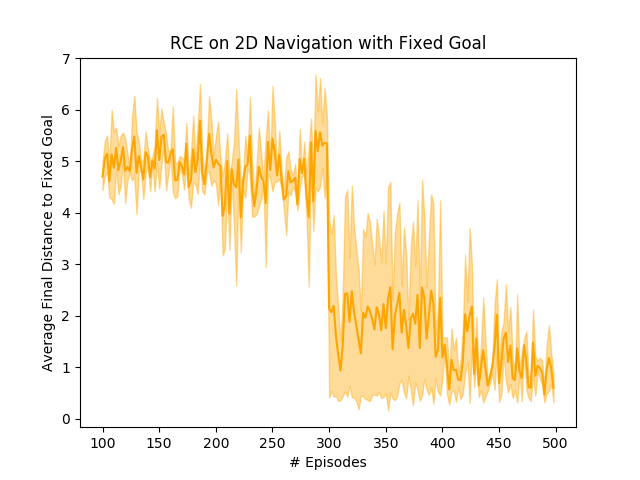
\includegraphics[width=0.8\linewidth]{img/solar/2dnav-rce.png}
    \caption{On 2D navigation with the goal fixed to the bottom right, RCE is able to successfully learning a policy for navigating to the goal.}
    \label{fig:pm-e2c}
\end{figure}

As mentioned in \autoref{sec:solar-experiments}, RCE was unable to make progress for the 2D navigation task, though we were able to get more successful results by fixing the position of the goal to the bottom right as is done in the image-based 2D navigation task considered in E2C \citep{e2c} and RCE \citep{rce}. \autoref{fig:pm-e2c} details this experiment, which we ran for three random seeds and report the mean and standard deviation of the average final distance to the goal as a function of the number of training episodes. This indicates that RCE can indeed solve some tasks from image observations, though we were unable to use RCE succesfully on any of the tasks we consider.

\subsection{Full Learning Progress of PPO}

In \autoref{fig:log-plots} we include the plots for the simulated tasks comparing \metabbr\ and PPO. Note that the x-axis is on a log scale, i.e., though our method is sometimes worse in final policy performance, we use one to three orders of magnitude fewer samples. This demonstrates our method's sample efficiency compared to model-free methods, while being able to solve complex image-based domains that are difficult for model-based methods.

\begin{figure}
    \centering
    \begin{subfigure}{0.32\linewidth}
        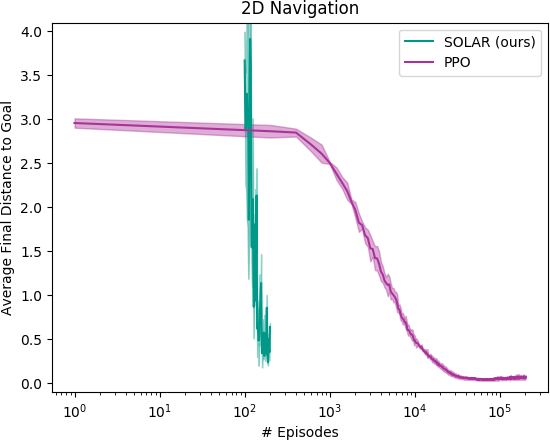
\includegraphics[width=0.9\linewidth]{img/solar/2dnav-log.png}
        \caption{}
    \end{subfigure}
    \begin{subfigure}{0.31\linewidth}
        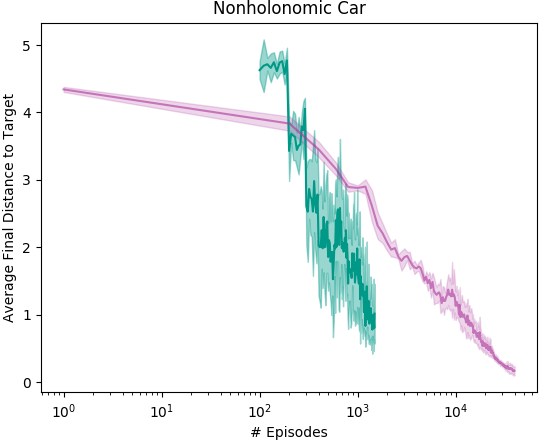
\includegraphics[width=0.9\linewidth]{img/solar/car-log.png}
        \caption{}
    \end{subfigure}
    \begin{subfigure}{0.33\linewidth}
        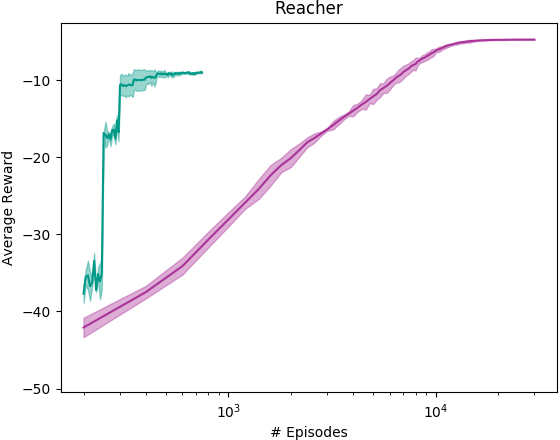
\includegraphics[width=0.9\linewidth]{img/solar/reacher-log.png}
        \caption{}
    \end{subfigure}
    \caption{(a)~Comparison of our method to PPO on the 2D navigation task presented in the paper. Our method uses roughly three orders of magnitude fewer samples to solve the task compared to PPO. (b)~On the car from images task, our method achieves slightly worse performance than PPO though with about 25 times fewer samples. (c)~Comparison of our method to PPO for the reacher task. Our method achieves worse final performance but uses about 40 times fewer samples than these methods.}
    \label{fig:log-plots}
\end{figure}